\documentclass{article}

\usepackage{graphicx} % Required for inserting images

\usepackage[T1]{fontenc}
\usepackage[utf8]{inputenc}
\usepackage{lmodern}
\usepackage[italian]{babel}
\usepackage{svg}
\usepackage{amssymb} %per i simboli matematici bellini
\usepackage{amsmath}%per l'environment split (dividere un'equazione su più righe) 
\usepackage{xcolor} %per i colori dentro lstlistings o s'incazza
\usepackage{listings}%per le parti di codice
\usepackage{float}
\usepackage{algorithm}
\usepackage{algpseudocode}
\usepackage{fancyhdr} %Per modificare il fondo pagina
\usepackage{makecell} %per mettere il testo di una cella su più righe
\usepackage{enumitem} % per le liste interrotte
\usepackage{hyperref} %Per fare i riferimenti. A cose normali verrebbero i link ipertestuali, per toglierli:
\hypersetup{
    colorlinks=true,
   % linkcolor=black,
    allcolors=black,
   % filecolor=magenta,      
   % urlcolor=cyan
   % citecolor=black
} 


%per avere il codice più bellino. 
\lstset{
  basicstyle=\ttfamily,
  columns=fullflexible,
  frame=single,
  breaklines=true,
  postbreak=\mbox{\textcolor{red}{$\hookrightarrow$}\space},
}


\floatname{algorithm}{Algoritmo}
\addto\captionsitalian{%
\renewcommand{\lstlistingname}{Listato}}
\newcommand{\algorithmautorefname}{Algoritmo}

%Per mettere in fondo altro oltre che il numero di pagina
\fancyhf{}
\rhead{}
\rfoot{Pagina \thepage}
\pagestyle{fancy}
\renewcommand{\footrulewidth}{0.4pt}

%\title{Relazione Laboratorio di  Automatica}
\title{Controllo tramite Potenziali Artificiali di un Rover con marker ArUco}
\author{Elena Bellanova \\ Giulio Beltrami \\ Marco Minarelli}
%\date{March 2024}

\date{}


\begin{document}
\begin{titlepage}
    \begin{center}
        \textsc{\Large Universit\`a degli Studi di Firenze}\medskip
	    \\ [1.0cm]
		% Change to your faculty if needed
		
\includegraphics[width=25mm]{img/stemma}\\[.5cm]
		 \textsc{ Ingegneria Elettrica e dell'Automazione \\ Curriculum Automazione e Robotica}\medskip\\
		 \rule{50mm}{0.01mm}\medskip\\
		Elaborato di Laboratorio di Automatica \medskip\\
    \LARGE \textbf{ Controllo in Sliding Mode di un Rover con waypoint ArUco } 
    \normalsize  \vspace*{5\baselineskip}
    \medskip\\
       
         \end{center}
          \makeatletter
    \begin{minipage}[t]{65mm}
   \raggedright
   {\it Studenti}\newline
    \@author
   \end{minipage}%
		\makeatother
		
   \vfill
  \begin{center}
    \rule{40mm}{0.01mm}\\
    {Anno Accademico 2023/2024}
  \end{center}
\end{titlepage} 


%\maketitle
\tableofcontents

\clearpage
%descrizione del problema, obiettivo e come è strutturata la relazione
\section{Introduzione}
L'obiettivo del progetto è far convergere il rover a rette le cui equazioni sono dinamicamente calcolate, evitando al contempo gli ostacoli inseriti nelle traiettorie che vogliamo far percorrere al rover.  Le rette sono definite a  partire da marker ArUco i quali vengono riconosciuti tramite tecniche di visione artificiale, mentre per la parte di obstacle avoidance sono stati implementati algoritmi che fanno uso di potenziali artificiali (Artificial Potential Field). In particolare sono stati implementati un potenziale attrattivo, che porta a far convergere il sistema al goal prefissato e uno repulsivo, che tiene lontano il rover dagli ostacoli.\\
In particolare la relazione è stata suddivisa in: "Descrizione tecnica del veicolo" (\autoref{sec:desc_tec}) dove vengono descritte tutte le componenti; "Premesse Teoriche" (\autoref{sec:prem_teo}) dove vengono illustrati i fondamenti teorici degli algoritmi utilizzati; "Implementazione" (\autoref{sec:impl}) dove viene riportato il lavoro svolto relativo alla codifica dei suddetti algoritmi; "Risultati" (\autoref{sec:res}) dove vengono tracciati i grafici delle traiettorie ottenute. Infine nella sezione "Conclusioni e Sviluppi futuri" (\autoref{sec:concl}) vengono proposte possibili migliorie al sistema e valutato se gli obiettivi sono stati raggiunti.


%  descrizione robot
\section{Descrizione tecnica del veicolo} 
\label{sec:desc_tec}
Il rover utilizzato è un robot a quattro ruote ricavato da una macchina giocattolo RC, attuato da due motori: uno per lo sterzo mentre l'altro per la trazione. Di seguito vengono descritti i principali componenti e sensori utilizzati. La parte software del rover è controllata tramite il modulo Nvidia Jetson AGX Orin.

\subsection{Nvidia Jetson AGX Orion}
Il kit per sviluppatori NVIDIA Jetson AGX Orin  \cite{Nvidia} e tutti i moduli Jetson Orin condividono un'unica architettura SoC, consentendo di emulare prestazioni e potenza per qualsiasi modulo. È configurato per impostazione predefinita per coloro che utilizzano i moduli della serie Jetson AGX Orin, ma può essere facilmente riprogrammato per emulare i moduli della serie Jetson Orin NX o Jetson Orin Nano. \\
La scheda carrier inclusa espone molte interfacce hardware standard, consentendo una piattaforma altamente flessibile ed estensibile per la prototipazione rapida.

\subsection{ZED}
La fotocamera ZED \cite{ZED} è progettata per replicare il funzionamento della visione umana. Utilizzando le due camere e la triangolazione, la ZED fornisce una comprensione tridimensionale della scena osservata.
Le caratteristiche principali sono:
\begin{itemize}
    \item Piattaforma di percezione spaziale end-to-end per capacità di rilevamento simili a quelle umane;
    \item Prestazioni in tempo reale, infatti tutti gli algoritmi dell'SDK ZED sono progettati e ottimizzati per funzionare in tempo reale;
    \item Ampia gamma di piattaforme supportate, dai PC desktop ai PC embedded.
\end{itemize}

\subsection{LiDAR}
L’acronimo LiDAR (Light Detection And Ranging) \cite{lidar} \cite{lidar2} identifica la tecnologia che  misura la distanza da un oggetto illuminandolo con una luce laser e che è  in grado di restituire informazioni tridimensionali ad alta risoluzione sull’ambiente circostante. Un LiDAR utilizza tipicamente diversi componenti: laser, fotorilevatori e circuiti integrati di lettura con capacità di tempo di volo per misurare la distanza illuminando un bersaglio e analizzando la luce riflessa.
Di base il LIDAR è una tecnica simile ad un radar basata sul principio dell'eco.\\
L’utilizzo della tecnologia LiDAR comporta diversi vantaggi legati alla sua implementazione:
\begin{itemize}
\item Garantisce una misurazione veloce e precisa;
\item Ampia risoluzione: la luce ha lunghezze d’onda minori rispetto alle onde radio e questo aumenta la risoluzione del rilevamento e permette quindi di classificare meglio gli oggetti;
\item Semplicità e la facilità d’utilizzo.
\end{itemize}

\begin{figure} [H]
    \centering
    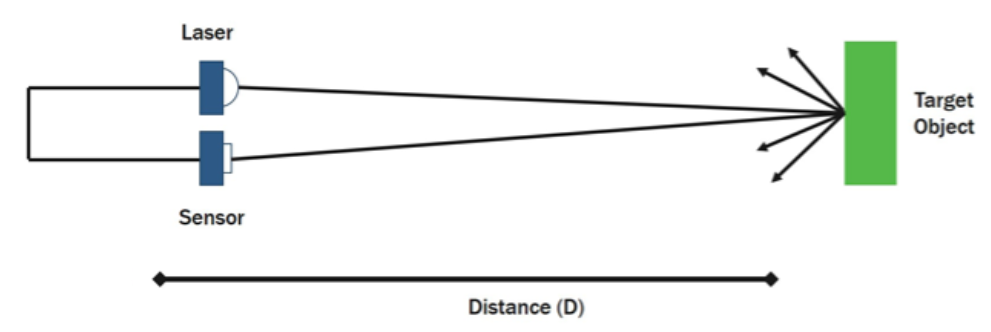
\includegraphics[width=0.5\linewidth]{img/Lidar.PNG}
    \caption{Funzionamento LiDAR}
    \label{fig:Lidar}
\end{figure}
\noindent
In tale applicazione il LiDAR utilizzato è della marca YDLiDAR, modello G4, che ha le seguenti caratteristiche:
\begin{itemize}
\item Capacità di scansione a 360° (2D) entrambi i sensi di rotazione;
\item Offre una velocità di scansione di 9.000 scansioni al secondo con una portata di 16 m;
\item Comunicazione dati wireless.
\end{itemize}







%smc/algoritmi,
\section{Premesse teoriche}
\label{sec:prem_teo}
\subsection{ArUco marker}
Un marcatore ArUco \cite{ArUco} è un marcatore quadrato sintetico composto da un ampio bordo nero e da una matrice binaria interna che ne determina l'identificatore.\\ 
\`E importante notare che l'identificatore del marcatore non si ottiene convertendo la codifica binaria in un numero a base decimale. Ciò non è possibile poiché per dimensioni elevate dei marcatori il numero di bit è troppo elevato e gestire numeri così grandi non è pratico. Invece, l'identificatore del marcatore è semplicemente l'indice del marcatore all'interno del dizionario a cui appartiene.
Il bordo nero ne facilita il rapido rilevamento nell'immagine e la codifica binaria ne consente l'identificazione, l'applicazione di tecniche di rilevamento e la correzione degli errori. La dimensione del marcatore determina la dimensione della matrice interna, ad esempio un marker di dimensione 6x6 è composto da 36 bit.\\
I markers vengono raggruppati in set, chiamati dizionari, in funzione della dimensione che determina anche la grandezza della matrice interna. 
Un marker può essere trovato ruotato nell'ambiente, tuttavia è necessario che il processo di rilevamento sia in grado di determinare la sua rotazione originaria, in modo che ogni angolo venga identificato in modo inequivocabile.\\
I marcatori ArUco sono progettati con un algoritmo che può essere matematicamente dimostrato per ottimizzare la distanza tra i marcatori, il che significa che riduce al minimo la possibilità di identificare erroneamente un marcatore per un altro se uno o pochi bit non vengono riconosciuti correttamente.\\
Una volta acquisita l’immagine contenente uno o più markers, il processo di detection viene effettuato tramite 2 step principali. \\
Nel primo step si effettua una detection cercando di trovare, all’interno dell’immagine, delle forme quadrate candidate ad essere possibili markers.\\ 
Nel secondo step è necessario prima trovare gli angoli del marcatore, correggere la distorsione prospettica per ottenere un'immagine che sembri come se il marcatore fosse visto dall'alto, dividere l'immagine risultante in una griglia e confrontare questa griglia di celle bianche e nere con il dizionario fornito per scoprire se esiste una corrispondenza.
\\
\\
\begin{figure} [H]
    \centering
    
\includegraphics[width=0.5\linewidth]{img/ArUco.jpeg}
    \caption{Esempio di marcatori ArUco}
    \label{fig:ArUco}
\end{figure}

\subsection{ROS2}
Robot Operating System (ROS)\cite{ROS2} \cite{RobOpeSys} è un framework mediante il quale è possibile creare applicazioni robotiche scalabili per robot. Lo scopo di ROS è scomporre il software complesso in parti più piccole e più gestibili, semplificando il processo di sviluppo in quanto fornisce un'interfaccia unificata per la comunicazione tra diversi processi su cui possono essere eseguiti diversi componenti software del robot.\\ 
Inoltre, ROS dispone di un ampio ecosistema di pacchetti di sensori, controllo e algoritmi.\\
ROS ha anche un concetto chiamato server dei parametri, sul quale i parametri globali possono essere memorizzati e accessibili da tutti i nodi. \\
Un nodo non è altro che un file eseguibile all'interno di un ROS package. I nodi del ROS usano una libreria del ROS client per comunicare con altri nodi. I nodi possono pubblicare o iscriversi a un Topic. 
Il nodo è importante un'unità organizzativa che consente a un utente di ragionare su a sistema complesso. L'architettura anonima publish-subscribe consente una comunicazione many-to-many. Uno sviluppatore può osservare eventuali messaggi che passano su un topic creando una sottoscrizione a quell'argomento senza alcuna modifica.
Per governare la comunicazione è necessario stabilire le specifiche dell'interfaccia. Questi messaggi definiscono la
semantica dei dati scambiati. I messaggi definiti vengono comunicati
tra i componenti in modo asincrono, creando un sistema basato sugli eventi. Con questo approccio, un'applicazione può
lavorare nei molteplici domini temporali che derivano dalla combinazione di dispositivi fisici con una serie di componenti software;
ognuno dei quali può avere una propria frequenza di erogazione
dati, accettare comandi o segnalare eventi.

 \subsection{Artificial Potential Field} \label{APF}
Il metodo dei Campi Potenziali Artificiali (o in inglese "Artificial Potential Field", da cui l'acronimo APF), presentato per la prima volta in \cite{khatibAPF}, è un 
metodo per la pianificazione del moto. Si considera il robot come una particella che si muove in un campo potenziale artificiale, il quale è a sua volta la somma di due 
campi: un campo attrattivo (che attrae il robot verso il goal) e un campo repulsivo (che allontana il robot dagli ostacoli). \\
Quindi, data la configurazione del robot $\boldsymbol{q}$, il campo totale è dato da 
\begin{equation}
  J(\boldsymbol{q}) = k_a J_{att}(\boldsymbol{q}) + k_r J_{rep}(\boldsymbol{q}), \: k_a > 0, \: k_r > 0
\end{equation}
e la direzione che il robot dovrà prendere (quindi la "forza" agente sul robot) è data da 
\begin{equation}
  -\frac{\partial  J(\boldsymbol{q})}{\partial \boldsymbol{q}} = -  k_a \frac{\partial  J_{att}(\boldsymbol{q})}{\partial \boldsymbol{q}} - k_r \frac{\partial  J_{rep}(\boldsymbol{q})}{\partial \boldsymbol{q}}
\end{equation}
Per la scelta dei campi attrattivi e repulsivi si può fare rifermiento a \cite{libroRobotica}. Nel nostro caso è stato scelto un potenziale attrattivo Huber-like: 
\begin{equation}
  \begin{cases}
    \frac{1}{2} || \boldsymbol{q} - \boldsymbol{q_G}||^2 \: \: \:  \: \: \: & se \: || \boldsymbol{q} - \boldsymbol{q_G}|| \leq \delta \\
    \delta || \boldsymbol{q} - \boldsymbol{q_G}|| - \frac{1}{2}\delta^2 \: \: \: & altrimenti
  \end{cases} 
  \Rightarrow \boldsymbol{f_{attr}} = 
  \begin{cases}
   \boldsymbol{q} - \boldsymbol{q_G}\: \: \:  & se \: || \boldsymbol{q} - \boldsymbol{q_G}|| \leq \delta \\
    \frac{ \boldsymbol{q} - \boldsymbol{q_G}}{|| \boldsymbol{q} - \boldsymbol{q_G}||}  \: \: \: & altrimenti
  \end{cases} 
\end{equation}
dove con $  \boldsymbol{q_G} $ si indica la configurazione obbiettivo e con $ \delta  $ la distanza di switch tra un potenziale e l'altro. 
Per il campo repulsivo dell'ostacolo $i$-esimo, invece è stato scelto
\begin{equation}
  \begin{cases}
    \frac{1}{\gamma} (\frac{a}{d( \boldsymbol{q},  \boldsymbol{q_{obs_i})}} - \frac{1}{\delta_0})^\gamma \: \: \:  & se \: d( \boldsymbol{q},  \boldsymbol{q_{obs_i}}) \leq \delta_0 \\
    0  \: \: \:  & altrimenti
  \end{cases} 
\end{equation}
%\begin{equation}
% \begin{cases}
%    \frac{1}{\gamma} (\frac{a}{d( \boldsymbol{q},  %\boldsymbol{q_{obs_i}}} - \frac{1}{\delta_0})^\gamma \: \: \:  % & se \: d( \boldsymbol{q},  \boldsymbol{q_{obs_i}}) \leq %\delta_0 \\
%    0  \: \: \:  & altrimenti
%  \end{cases}  \\
%  \Rightarrow \boldsymbol{f_{rep}} = 
%  \begin{cases}
  
%  \begin{split}
%   \frac{1}{d( \boldsymbol{q},  \boldsymbol{q_{obs_i}} )^2} ( \frac{1}{d( \boldsymbol{q},  \boldsymbol{q_{obs_i}}} - \frac{1}{\delta_0})^{\gamma -1}& \nabla d( \boldsymbol{q},  \boldsymbol{q_{obs_i}} ) \\   \: \: \: & se \:  d( \boldsymbol{q},  \boldsymbol{q_{obs_i}} ) \leq \delta_0 
%   \end{split} \\
%    \frac{ \boldsymbol{q} - \boldsymbol{q_G}}{|| \boldsymbol{q} - \boldsymbol{q_G}||}  \: \: \: altrimenti
%  \end{cases} 
%\end{equation}

\begin{equation*}
\Rightarrow \boldsymbol{f_{rep}} = 
\begin{cases}

  \frac{1}{d( \boldsymbol{q},  \boldsymbol{q_{obs_i}} )^2} ( \frac{1}{d( \boldsymbol{q},  \boldsymbol{q_{obs_i}}} - \frac{1}{\delta_0})^{\gamma -1} \nabla d( \boldsymbol{q},  \boldsymbol{q_{obs_i}} )   \: \: \: & se \: d( \boldsymbol{q},  \boldsymbol{q_{obs_i}} ) \leq \delta_0 
   \\
\frac{ \boldsymbol{q} - \boldsymbol{q_G}}{|| \boldsymbol{q} - \boldsymbol{q_G}||} \: \: \:  & altrimenti
  \end{cases} 
\end{equation*}
con $ \gamma = 2$, $ \boldsymbol{q_{obs_i}} $ la rappresentazione dell'ostacolo nello spazio delle configurazioni, con $ d( \boldsymbol{q},  \boldsymbol{q_{obs_i}}) $ la
distanza tra il robot e l'ostacolo e infine con $ \delta_0 $ la soglia sopra la quale l'ostacolo non esercita nessuna influenza sul robot.
Uno dei vantaggi dell'algoritmo APF è che può essere impiegato per effettuare planning online, quindi senza conoscenza a priori della mappa e delle posizioni (o della 
forma) degli ostacoli. Inoltre, grazie alla soglia sulla distanza degli ostacoli presente nel potenziale repulsivo, è possibile associare un potenziale ad ogni oggetto rilevato entro tale distanza invece che cercare di ricostruirne la forma.

\subsubsection{LOS APF}
 Al fine di vincolare il veicolo a rimanere in una regione limitata attorno al percorso diretto tra due punti di passaggio consecutivi, il metodo precedente viene quindi modificato utilizzando un approccio di Line Of Sight(LOS) \cite{LOSAPF}. In questo caso il potenziale attrattivo non è più associato al waypoint attuale ma ad un punto LOS.
Il calcolo del punto LOS si basa sull'intersezione tra il cerchio di raggio $r$, centrato sulla posizione del rover e la linea $D_k$, dove $D_k$ è la linea retta che unisce le coordinate precedente e quelle attuali. Se esistono due punti di intersezione, il punto LOS viene scelto come soluzione più vicina al punto di passaggio corrente. Se non c'è soluzione (cioè il rover si trova a una distanza maggiore di $r$ dalla linea retta tra il punto di passaggio precedente e quello attuale), il punto LOS viene scelto come proiezione ortogonale della posizione della barca sulla linea.
Poiché il punto LOS, con il suo potenziale associato, giace sempre su $D_k$, questo potenziale in movimento attirerà il rover verso la linea retta tra i due punti di passaggio e costringerà il veicolo a rimanere in una fascia limitata di larghezza inferiore o uguale a $r$. 
Il valore del punto LOS viene aggiornato ogni volta che viene eseguito l'algoritmo.
\begin{figure} [H]
    \centering
    \includesvg[width=0.5\linewidth]{img/LOSAPFDisegno}
    \caption{Tecnica di intersezione}
    \label{fig:LOS}
\end{figure}

\subsection{Controllori PID}
    \begin{figure}[h]
      \centering
      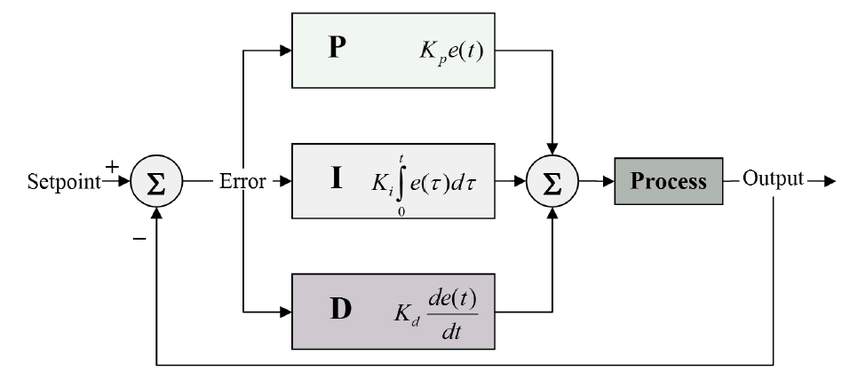
\includegraphics[width=0.8\textwidth]{img/PID.png}
      \caption{Rappresentazione a blocchi di un controllore PID}
      \label{img:PID}
    \end{figure}
    \noindent
  Si consideri un generico sistema $P(s)$ da controllare attraverso un controllore $C(s)$, come mostrato in \autoref{img:PID}. Esistono varie tecniche per realizzare il controllore; una delle più utilizzate è la tecnica PID, dove l'acronimo definisce le tre leggi di controllo Proporzionale, Integrale e Derivativo. L'errore misurato, dato dalla differenza tra il riferimento e l'uscita effettiva 
    del sistema, è l'ingresso del controllore, il quale genera un segnale di uscita $u$ composto dalle tre componenti 
    proporzionale, integrale e derivativa:
    \begin{displaymath}
      \boldsymbol{u} = K_P  \boldsymbol{e}  + K_D  \dot{ \boldsymbol{e}} + K_I \int_{0}^t  \boldsymbol{e}(\tau) d\tau 
    \end{displaymath}
  La funzione di trasferimento del sistema $C_{PID}(s)$ vale quindi 
  \begin{displaymath}
    C_{PID}(s)=K_P + \frac{K_I}{s}+ K_Ds = \frac{K_Ds^2 + K_Ps + K_I}{s}
  \end{displaymath}
  Le azioni dei tre contributi sono le seguenti:
  \begin{itemize}
    \item Il contributo proporzionale permette di migliorare la prontezza della risposta e ridurre l'errore a regime permanente
    \item Il contributo integrale permette eliminare l'errore a regime permanente peggiorando però la risposta transitoria
    \item Il contributo derivativo permette di aumentare la stabilità del sistema.
  \end{itemize}

\subsubsection{Schemi anti wind-up}
Il fenomeno del wind-up è dovuto all’azione integrale. Questo fenomeno si innesca quando i sistemi di attuazione che trasformano il segnale di comando nell’azione di controllo vanno in saturazione. Questo accade quando $e(t)$, che a causa della saturazione  rimane costante in segno, viene integrato.\\
Quando poi cambia il segnale di riferimento, $e(t)$ cambia segno ma prima di osservare una variazione del segnale di comando le componenti integrali del PID si devono scaricare così da uscire dalla saturazione. Questo può richiedere tempi lunghi con una conseguente perdita di reattività. \\
Si usano degli schemi anti wind- up per prevenire questo fenomeno. Una delle tecniche anti wind-up più nota in letteratura  è il  "Clamping". \\
 \begin{figure} [H]
    \centering
    \fontsize{8}{10}\selectfont
    \includesvg[width=1\linewidth]{img/PIDAntiWindupClamping}
    \caption{Schema PID}
    \label{img:antiwindup}
\end{figure}
\noindent
In questa tecnica il segnale di comando viene confrontato con le due soglie scelte come valore massimo e minimo di saturazione del PID. Quando il sistema si trova in saturazione non viene aggiornata la somma dell'azione integrale, in tale modo la somma rimane invariata rispetto agli istanti precedenti. Se invece siamo all'interno dell'intervallo scelto la somma viene aggiornata con un nuovo valore. 


% nodi, linguaggio, messaggi custom
\section{Implementazione}
\subsection{Nodo di visione}
Gli obiettivi del nodo visione sono:
\begin{enumerate}
  \item riconoscere nell'immagine i markers ArUco;
  \item localizzarli nella mappa;
  \item ricavare l'id del marker e quindi il coefficiente angolare della retta a cui il robot dovrà convergere.
\end{enumerate}
  Per quanto riguarda il primo punto, la libreria OpenCV \cite{opencv_library} mette a disposizione un modulo che permette di ricavare la posizione degli angoli del 
  marker e di ricavare l'id associato. \\
  Riguardo il secondo punto, supponendo di conoscere la matrice di calibrazione $K$ della camera \cite{multiple_view} e la posizione dell'ArUco in coordinate omogenee 
  $p_w = (X \: Y \: Z \: 1 )^T$, se definiamo il punto immagine come in coordinate pixel $ p_c =  (u \: v \: 1)^T$ si ottiene 
    \begin{equation}
    p_c \propto K \Pi [R | \boldsymbol{t}] p_w  \Rightarrow
     \begin{bmatrix}
           u \\
           v \\
           1
        \end{bmatrix}
         \propto 
         \begin{bmatrix}
           f_x & \sigma & c_x \\
           0 & f_y & c_y \\
           0 & 0 & 1 
         \end{bmatrix}
          \begin{bmatrix}
           1 & 0 & 0 & 0 \\
           0 & 1 & 0 & 0 \\
           0 & 0 & 1 & 0
         \end{bmatrix}
         \begin{bmatrix}
           r_{11} & r_{12} & r_{13} & t_1 \\
           r_{21} & r_{22} & r_{23} & t_2 \\
           r_{31} & r_{32} & r_{33} & t_3  \\
           0 & 0 & 0 & 1
         \end{bmatrix}
         \begin{bmatrix}
           X \\
           Y \\
           Z \\
           1
    \end{bmatrix}
  \end{equation}
  con $R$ matrice di rotazione e $ \boldsymbol{t}$ vettore che indica la traslazione tra la camera e il marker; calcolando questi due elementi si può ricavare la 
  posa del target in terna camera. Per risolvere questo problema sono stati realizzati vari algoritmi \cite{marchand2015pose}, i quali possono essere richiamati dalla 
  funzione \texttt{solve\_PnP()} della libreria. Nello specifico in \cite{infinitesimal} è proposto un metodo per risolvere il problema nel caso il target siano dei
  marker. \\
  La matrice di trasformazione dalla terna Robot alla terna camera è data da \footnote{In realtà la matrice di trasformazione dovrebbe essere $T^R_C = \begin{bmatrix} 0 & 0 & 1 & 0 \\ -1 & 0 & 0 & 0 \\ 0 & -1 & 0 & 0 \\ 0 & 0 & 0 & 1 \end{bmatrix} $. Ma, dato che la camera è ruotata di $180^{\circ}$ si ottiene la matrice sopra riportata. }   
\begin{equation}
T^R_C = \begin{bmatrix} 0 & 0 & 1 & 0 \\ 1 & 0 & 0 & 0 \\ 0 & 1 & 0 & 0 \\ 0 & 0 & 0 & 1 \end{bmatrix} 
\end{equation}\\ mentre la matrice di trasformazione dalla terna camera alla terna marker da 
\begin{equation}
T^C_M = \begin{bmatrix} R & \boldsymbol{t} \\ \begin{matrix} 0 & 0  & 0 \end{matrix} & 1 \end{bmatrix}
\end{equation}
  A partire quindi dalla posa del marker rispetto a camera e dalla posa della camera in terna fissa si può ottenere la posizione in terna fissa del marker $(x_A, y_A)$.\\
  In terna marker i corner, a destra e a sinistra, hanno rispettivamente coordinate
  \[
     {\boldsymbol{x_r}}=\begin{pmatrix} \frac{Markersize}{2} \\ \frac{Markersize}{2} \\ 0 \end{pmatrix} \ \ \ \;
     {\boldsymbol{x_l}}=\begin{pmatrix} -\frac{Markersize}{2} \\ \frac{Markersize}{2} \\ 0 \end{pmatrix}
  \]
  Si può quindi calcolare le coordinate di tali punti in terna camera calcolando $T^R_C \cdot T^C_M \cdot P_{corner}$; a questo punto è possibile ottenere le coordinate
  dei corner in terna fissa. Da queste coordinate si può ricavare l'equazione della retta $r_{corner}: y = m_{corner} x + q_{corner}$ passante per i corner, sempre in 
  terna fissa. \\
  L'id del marker identifica la direzione desiderata cioé la rotazione desiderata di $r_{corner}$ attorno al punto $(x_A, y_A)$. A livello algoritmico, si considera
  il coefficiente angolare $m_{corner}$, si calcola il nuovo coefficiente angolare applicando la rotazione desiderata ed infine si impone che la nuova retta 
  passi per le coordinate del marker, imponendo cioé $q = y_A - m \cdot x_A$.
  
\subsection{Nodo di controllo}
\subsubsection{APF}
Per poter utilizzare tale tipologia di controllo bisogna calcolare il \textit{goal} dinamicamente, cioè calcolare l'intersezione tra la retta e il cerchio di raggio $r$. Ricordiamo che le coordinate $(x_r,y_r)$ coincidono con quelle del rover. \\
Si possono distinguere due casi, quello in cui la retta è definita come $y=mx+q$ e quello in cui si ha $x=cost$.\\
Riferendoci al primo caso, si imposta il sistema:
\begin{equation} 
\begin{cases}

    (x-x_r)^2+(y-y_r)^2=r^2
   \\
    y=mx+q 
  \end{cases} 
\end{equation}
si sostituisce la seconda equazione nella prima
\begin{equation*}
(x-x_r)^2+(mx+q-y_r)^2=r^2
\end{equation*}

\begin{equation}
\Rightarrow x^2+x_r^2-2xx_r+m^2x^2+q^2+y_r^2+2mxq-2mqy_r-2mxy_r-r^2=0
\end{equation}

\begin{equation*}
\Rightarrow \underbrace{(1+m^2)}_\text{a}x^2+\underbrace{(2mq-2x_r-2my_r)}_\text{b}x+\underbrace{(x_r^2+q^2+y_r^2-2qy_r-r^2)}_\text{c}=0
\end{equation*}
Definiamo $\Delta=b^2-4ac=(2mq-2x_r-2my_r)^2-4(1+m^2)(x_r^2+q^2+y_r^2-2qy_r-r^2)$. \\Se:
\begin{itemize}
    \item $\Delta>0$ si hanno due soluzioni
        \begin{equation}
        x_1=\frac{-(2mq-2x_r-2my_r)+\sqrt{2mq-2x_r-2my_r)^2-4(1+m^2)(x_r^2+q^2+y_r^2-2qy_r-r^2)}}{2(1+m^2)}
        \end{equation}
        \\
        \begin{equation}
        x_2=\frac{-(2mq-2x_r-2my_r)-\sqrt{2mq-2x_r-2my_r)^2-4(1+m^2)(x_r^2+q^2+y_r^2-2qy_r-r^2)}}{2(1+m^2)}
        \end{equation}
        Se la distanza risulta maggiore del raggio $r$, si sceglie la soluzione più lontana rispetto alla posizione dell'ArUco.
        Nel caso in cui invece la distanza risulti minore del raggio si sceglie 
        \begin{itemize}
            \item quella con il coefficiente angolare $m$ minore nel caso in cui il rover giri a destra
            \item quella con il coefficicnte angolare maggiore nel caso in cui il river giri a sinistra
        \end{itemize}
    \item $\Delta=0$ si ha una sola soluzione
    \begin{equation}
        x_d=\frac{-(2mq-2x_r-2my_r)}{2(1+m^2)}
        \end{equation}
    \item $\Delta<0$ non si hanno soluzioni, per cui usiamo la proiezione ortogonale tra la retta $y=mx+q$ e la retta passante per le coordinate $(x_r, y_r)$ del rover.
\end{itemize}
Riferendoci al secondo caso invece, si imposta il sistema:

\begin{equation} 
\begin{cases}

    (x-x_r)^2+(y-y_r)^2=r^2
   \\
    x=x_a 
  \end{cases} 
\end{equation}
si sostituisce la seconda equazione nella prima
\begin{equation*}
(x_a-x_r)^2+(y-y_r)^2=r^2
\end{equation*}

\begin{equation}
\Rightarrow x_a^2+x_r^2-2x_ax_r+y^2+y_r^2-2yy_r-r^2=0
\end{equation}

\begin{equation*}
\Rightarrow y^2+\underbrace{(-2y_r)}_\text{b}y+\underbrace{(x_r^2+x_a^2-2x_ax_r+y_r^2-r^2)}_\text{c}=0
\end{equation*}
Definiamo $\Delta=b^2-4ac=(-2y_r)^2-4(x_r^2+x_a^2-2x_ax_r+y_r^2-r^2)$. \\Se:
\begin{itemize}
    \item $\Delta>0$ si hanno due soluzioni
        \begin{equation}
        y_1=\frac{(2y_r)+\sqrt{(-2y_r)^2-4(x_r^2+x_a^2-2x_ax_r+y_r^2-r^2)}}{2}
        \end{equation}
        \\
        \begin{equation}
        y_2=\frac{(2y_r)-\sqrt{(-2y_r)^2-4(x_r^2+x_a^2-2x_ax_r+y_r^2-r^2)}}{2}
        \end{equation}
  Se la distanza risulta maggiore del raggio $r$, si sceglie la soluzione più lontana rispetto alla posizione dell'ArUco.
        Nel caso in cui invece la distanza risulti minore del raggio si sceglie 
        \begin{itemize}
            \item quella con il coefficiente angolare $m$ minore nel caso in cui il rover giri a destra
            \item quella con il coefficicnte angolare maggiore nel caso in cui il river giri a sinistra
        \end{itemize}    \item $\Delta=0$ si ha una sola soluzione
    \begin{equation}
        y_d=y_r
        \end{equation}
    \item $\Delta<0$ non si hanno soluzioni, per cui usiamo la proiezione ortogonale tra la retta $x=cost$ e la retta $y=cost$ pasante per $y_r$.
\end{itemize}
Il punto così ottenuto è il $\boldsymbol{q_G}$ della \autoref{APF}.
Si applicano quindi le formule viste in tale sottosezione con i seguenti parametri

\begin{table} [H]
    \centering
    \begin{tabular}{|cc|}
    \hline
        Parametro & Valore usato \\  \hline
        $k_a$ &      \\  \hline
        $k_r$ &    \\  \hline
        $\delta$ &    \\  \hline
        $\delta_0$ &    \\  \hline
    \end{tabular}
\end{table}
\subsubsection{SMC}
Come visto nella \autoref{SMC_Theory} per definire un controllo SMC si ha bisogno di una funzione $u$ che nel nostro caso è stata scelta seguendo \cite{algoSMC}: 
\begin{equation}
        u_i=-\rho_{i}sign(\sigma_i)\: \: \: \: \: \: \: \:i=1,2
\end{equation}
con $\rho_i>0 \: \: \:i=1,2$. \\
Definiti poi gli errori 
\begin{equation}
\begin{cases}
    e_1=x_d-x 
   \\
   e_2=y_d-y
   \\
   e_3=\theta_d-\theta
\end{cases} 
\end{equation}
le superfici di sliding sono
\begin{equation}
       \sigma_1=e_1 \ \ \ \ \ \ \ \ \sigma_2=e_3-\arcsin(f(e_2))
\end{equation} 
dove $f(e_2)=-\min({\delta_1|e_2|^{-1},\ \delta_2})$ con $\delta_1 \in (0,1)$, $\delta_2>0$.\\ Per ottenere i guadagni $\rho_1$ e $\rho_2$ si calcolano i parametri  $r_1$, $r_2$ e $r_3$ in tale modo
\begin{equation}
        r_1= \max\left\{\frac{\delta_1+d_1-d_3)\sqrt{1-\delta_1^{2}}}{1+d_3-d_1}v_{max}, \frac{(1+d_2)(\omega_{max}+\rho_2) \frac{\rho_1}{\rho_2}+d_2v_{max}}{1-d_1}\right\}
\end{equation}
\begin{equation}
        r_2= \min\left\{\frac{\delta_1-d_3\sqrt{1-\delta_1^{2}}}{d_3}v_{min}, \frac{\delta_1}{d_3}-v_{max}\sqrt{1-\delta_1^{2}}\right\}
\end{equation}
\begin{equation}
        r_3= \frac{\delta_1-d_3\sqrt{1-\delta_1^{2}}+\delta_2v_{max}+\delta_1v_{min}}{(1-d_2\sqrt{1-\delta_1^{2}})}
\end{equation}
e si sceglie $r_1<\rho_1<r_2$,\ \ $r_3<\rho_2$. Con tale scelta la dinamica dell'errore converge asintoticamente all'insieme
\begin{equation}
        D=\left\{(e_1,e_2,e_3) \in \mathbb{R}: e_1=0, \ \  |e_2|\le\delta_2^{-1}C, \ \ |e_3|\le \arcsin{(C)} \right\}
\end{equation}
con $C=\frac{d_3(\rho_1+v_{max}\sqrt{1-\delta_1^{2}})}{v_{min}}$.
\begin{figure} [H]
    \centering
    \includesvg[width=0.5\linewidth]{img/SMC}
    \caption{Sliding Mode Control}
    \label{fig:SMC}
\end{figure}


\subsection{Nodo convertitore}
Tale nodo è stato implementetato con lo scopo di ottenere la velocità angolare e lineare a partire dall'accelerazione e dallo sterzo. Dopo aver ricavato tali parametri questi vengono inviati al rover.\\
Tramite l'utilizzo di un PID è possibile passare dall'errore di velocità ad un valore di uscita in percentuale (\%), che ci permette di controllare la velocità del rover. Per settare i gudagni del PID è stato usata l'applicazione PID Tuner disponibile su MATLAB. Infatti, tramite l'Identification Toolbox di MATLAB è stato possibile definire, dati dei campioni ottenuti sperimentalmente dal rover, la risposta del sistema ad un gradino.\\ La conversione velocità angolare $\rightarrow$ accelerazione è stata implementata tramite l'uso della derivta discreta
\begin{equation}
\omega(t+1)=\frac{\theta(t)-\theta(t-1)}{\Delta{T}} \ \ \
\Rightarrow \ \ \ \theta(t+1)=\theta(t)+\omega(t)\Delta{T}.
\end{equation} 

\subsubsection{Filtro complementare}
Per ottenere un segnale di velocità longitudinale del rover è stato implementato un filtro complementare \cite{Filtrocompelmentare}. Questo sfrutta i dati della posizione stimata del rover e dal'accellerometro della ZED filtrandoli tramite l'utilizzo di un filtro passa basso e di un filtro passa alto. Più precisamente l'idea è quella di derivare i dati della posizione del rover per ottenere una stima della velocità che viene poi mandata al filtro passa basso, mentre per quanto riguarda i dati dell'accelerometro questi vengono integrati per ottenere sempre una stima della velocità che viene poi filtrata tramite filtro passa alto.
L'uscita è data dalla somma dei due segnali ottenuti dai filtri.
Provenendo da sensori diversi, le misurazioni della velocità di entrambi i rami presentano diverse perturbazioni del rumore.
\begin{figure} [H]
    \centering
    \includesvg[width=0.8\linewidth]{img/Filtro complementare}
    \caption{Filtro complementare}
    \label{fig:Filtro complementare}
\end{figure}


\section{Risultati}
\label{sec:res}
Le prove svolte, atte a testare il corretto funzionemaento del rover e delle tecniche di controllo implememntate, sono le seguenti:
\begin{enumerate}
  \item esecuzione di una traiettoria rettangolare 
  \item esecuzione di una greca 
  \item esecuzione di una traiettoria rettangolare con APF 
\end{enumerate}
 Implementando una funzione in grado di salvare in formato .csv i dati della posizione del rover, durante il suo movimento, è stato possibile realizzare un plot in cui si mostra la traiettoria desiderata (Ground trought) a confronto con quella realizzata dal rover (Robot trajectory).

\subsection{Traiettoria rettangolare}
Nella realizzazione di tale prova sono stati eseguti due giri del rettangolo.
\begin{figure} [H]
    \centering
    \includesvg[width=\linewidth]{img/Rectangular}
    \caption{Traiettorie rettangolari}
    \label{fig:rect}
\end{figure} 

\subsection{Traiettoria Greca}
Nel grafico sono state riportate le tre traiettorie effettuarte dal rover in tre prove differenti. 
\begin{figure} [H]
    \centering
    \includesvg[width=0.8\linewidth]{img/Greca}
    \caption{Traiettoria Greca}
    \label{fig:greca}
\end{figure} 


\subsection{Traiettoria rettangolare con APF}
Nel grafico sono state riportate le due traiettorie effettuarte dal rover in due prove differenti. 
\begin{figure} [H]
    \centering
    \includesvg[width=0.8\linewidth]{img/ObsAvoidance}
    \caption{Traiettoria rettangolare con APF}
    \label{fig:rectAPF}
\end{figure} 


\section{Conclusioni}
\label{sec:concl}

\subsection{Sviluppi Futuri}
  Possibili sviluppi futuri possono essere i seguenti: 
  \begin{itemize}
    \item Implementazione filtro di Kalman (Correzione - Predizione) per una migliore stima della velocità lineare
    \item Implementazione Firmware per poter utilizzare gli encoder presenti nei motori di sterzo e trazione
    \item Aggiungere un router Wi-Fi a bordo del rover così da semplificare la connessione
    \item Integrazione di una memoria SSD con maggiore capacità
  \end{itemize}
  
\subsection{Conclusioni}
  Gli obiettivi fissati sono stati raggiunti come dimostrato dai grafici, nonostante gli errori sulla posa introdotti dalla ZED. Il nodo di visione riesce correttamente ad individuare i marker e gli id ad essi associati, il nodo di controllo sceglie correttamente il punto a cui convergere tra i due proposti  e riesce a svoltare in modo smooth.
  Per quanto riguarda l'obstacle avoidance il sistema evita gli ostacoli la cui posizione è conosciuta a priori dimostrando la bontà dell'implementazione di APF, mentre non è stato possibile testare APF nel caso di ostacoli dinamici a causa della mancata comprensione del funzionamento del LiDAR. Il nodo convertitore, tramite l'utilizzo di due PID correttamente regolati, traduce con successo le grandezze solitamente utilizzate nel controllo dei veicoli ($v$ e $\omega$) nelle grandezze impiegate nel \texttt{dart\_wrapper}. 


\addcontentsline{toc}{section}{Bibliografia}
\nocite{*}
\bibliographystyle{ieeetr}
\bibliography{src/biblio}

\end{document}
